\documentclass[conference]{IEEEtran}
\IEEEoverridecommandlockouts
% The preceding line is only needed to identify funding in the first footnote. If that is unneeded, please comment it out.
\usepackage{cite}
\usepackage{amsmath,amssymb,amsfonts}
\usepackage{algorithmic}
\usepackage{graphicx}
\usepackage{lipsum}
\usepackage{textcomp}
\usepackage[section]{placeins}
\usepackage{xcolor}
\usepackage{fontawesome5}
\usepackage{hyperref}

\makeatletter
\newcommand{\github}[1]{%
   \href{#1}{\faGithubSquare}%
}
\makeatother
\def\BibTeX{{\rm B\kern-.05em{\sc i\kern-.025em b}\kern-.08em
    T\kern-.1667em\lower.7ex\hbox{E}\kern-.125emX}}
\begin{document}

\title{Reinforcement Learning Algorithms Applied to Grid World and Simple Pendulum\\
}

\author{\IEEEauthorblockN{Raghavendra S Navaratna}
rsn3@illinois.edu\\
Link to the repository:\href{https://github.com/uiuc-ae598-rl-2023-spring/hw1-dp-raghavvs}{\faGithubSquare}   \\ 
}

\maketitle

\section{Introduction}
This is a report on evaluating the model-based and model-free reinforcement algorithms applied to the grid world problem and a simple pendulum.

\section{Grid World}

\subsection{Policy Iteration Method}

Policy iteration is a model-based reinforcement learning algorithm that iteratively improves the policy and value function until convergence by alternating between policy evaluation and policy improvement. \cite{b1}

\begin{table}[h]
\caption{Hyperparameter values}
\renewcommand{\arraystretch}{1.5}
\centering
\begin{tabular}{|c|c|c|c|c|}
\hline
\textbf{Hyperparameter} &  \textbf{Values}  \\ \hline
\textbf{Gamma ($\gamma$)} & 0.95  \\ \hline
\textbf{Epsilon ($\epsilon$)} & 0.1  \\ \hline
\textbf{Alpha ($\alpha$)} & 0.5  \\ \hline
\textbf{Iterations} & 100 \\ \hline
\textbf{Threshold ($\theta$)} & 1e-8 \\ \hline
\end{tabular} \\
\label{tab:hyperparameters}
\end{table}

\begin{figure}[!htbp]
\centerline{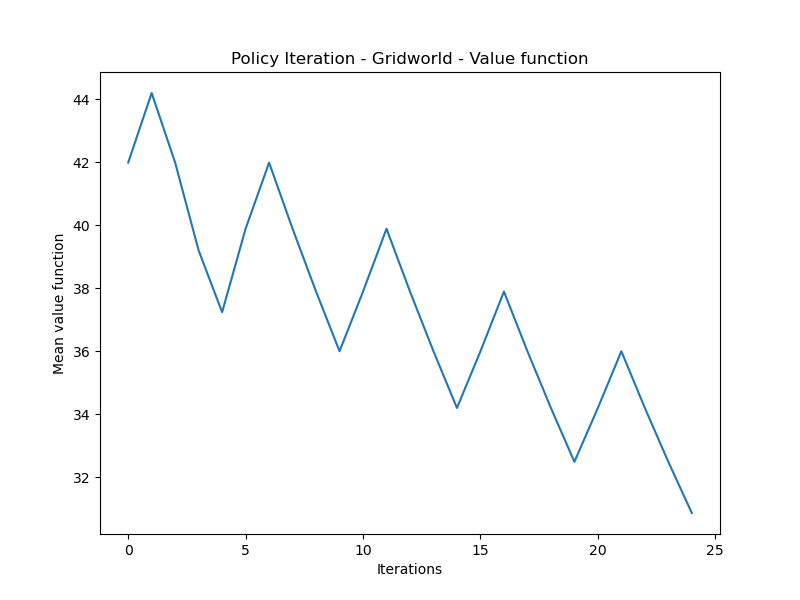
\includegraphics[width=3.5in]{g_pi_valfn_vs_iter.png}}
\caption{Mean Value Function vs. Number of Iterations}
\label{fig}
\end{figure}
\FloatBarrier

\begin{figure}[!htbp]
\centerline{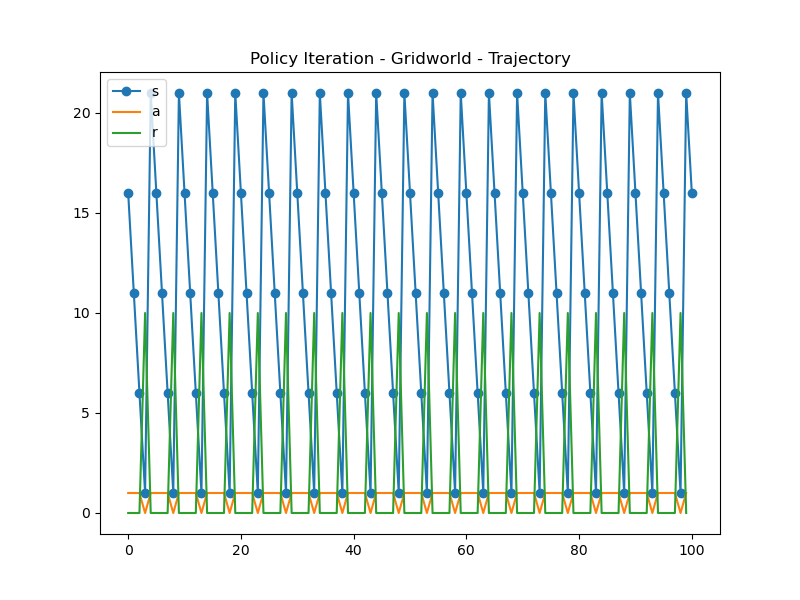
\includegraphics[width=3.5in]{g_pi_policy_vs_trajec.png}}
\caption{Policy vs. Trajectory}
\label{fig}
\end{figure}
\FloatBarrier

\subsection{Value Iteration Method}

Value iteration is a dynamic programming algorithm that computes the optimal value function by iteratively updating state values based on the maximum expected future reward achievable from each state. It converges to the optimal policy after a finite number of iterations. \cite{b1}

\begin{figure}[!htbp]
\centerline{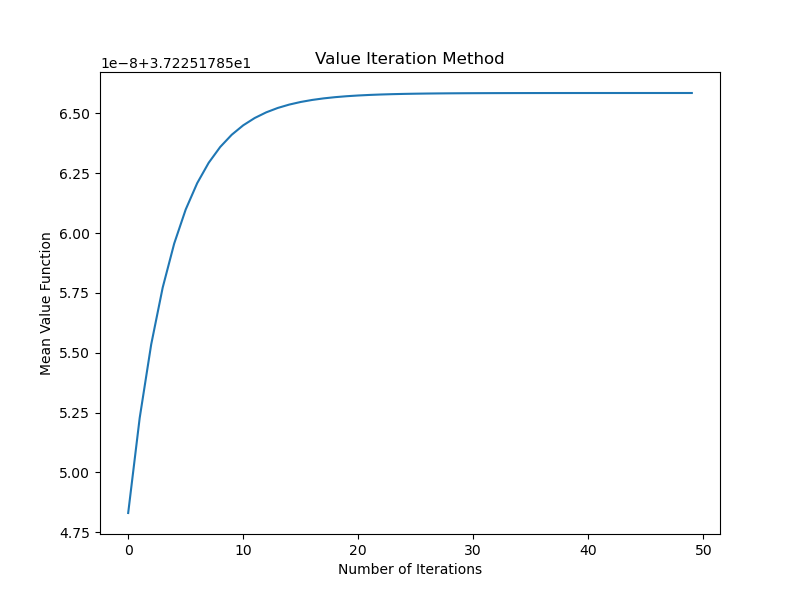
\includegraphics[width=3.5in]{g_vi_valfn_vs_iter.png}}
\caption{Mean Value Function vs. Number of Iterations}
\label{fig}
\end{figure}
\FloatBarrier

\begin{figure}[!htbp]
\centerline{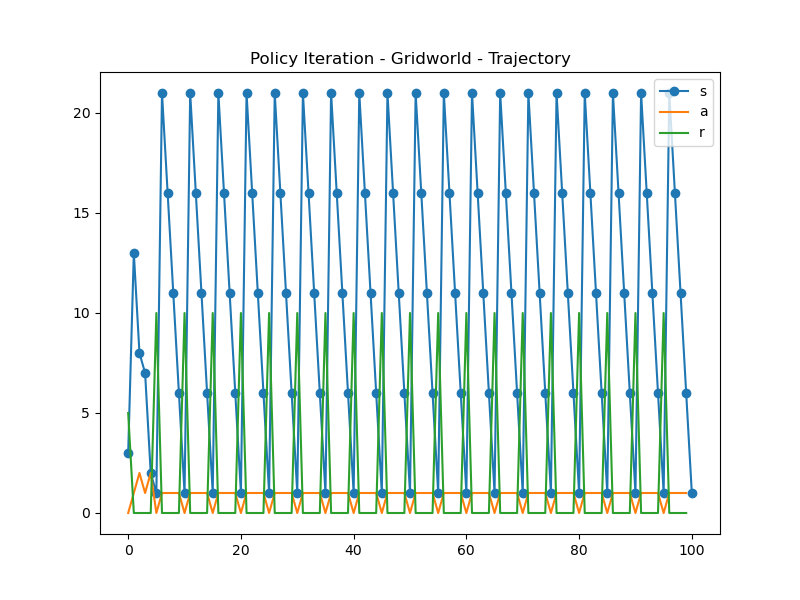
\includegraphics[width=3.5in]{g_vi_policy_vs_trajec.png}}
\caption{Policy vs. Trajectory}
\label{fig}
\end{figure}
\FloatBarrier

\subsection{SARSA}

SARSA (State-Action-Reward-State-Action) is a model-free reinforcement learning algorithm used for estimating the Q-values of a policy. It updates the Q-value of the current state-action pair based on the reward obtained and the Q-value of the next state-action pair, using the current policy to select the next action. \cite{b1}

\begin{table}[h]
\caption{Hyperparameter values}
\renewcommand{\arraystretch}{1.5}
\centering
\begin{tabular}{|c|c|c|c|c|}
\hline
\textbf{Hyperparameter} &  \textbf{Values}  \\ \hline
\textbf{Gamma ($\gamma$)} & 0.95  \\ \hline
\textbf{Epsilon ($\epsilon$)} & 0 - 1  \\ \hline
\textbf{Alpha ($\alpha$)} & 0.2 - 1  \\ \hline
\textbf{Iterations} & 100 \\ \hline
\textbf{Episodes} & 500  \\ \hline
\textbf{Threshold ($\theta$)} & 1e-8 \\ \hline
\end{tabular} \\
\label{tab:hyperparameters}
\end{table}

\begin{figure}[!htbp]
\centerline{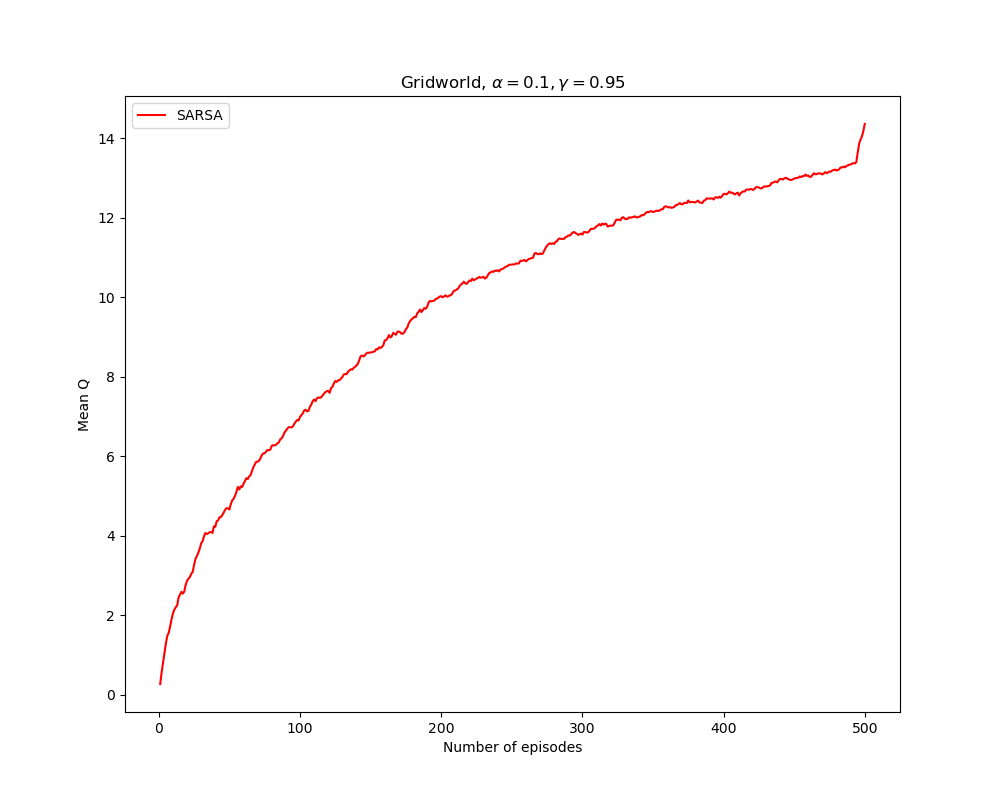
\includegraphics[width=3.5in]{g_sarsa_learning_curve}}
\caption{Learning Curve - Mean Value Function vs. Number of Episodes}
\label{fig}
\end{figure}
\FloatBarrier

\begin{figure}[!htbp]
\centerline{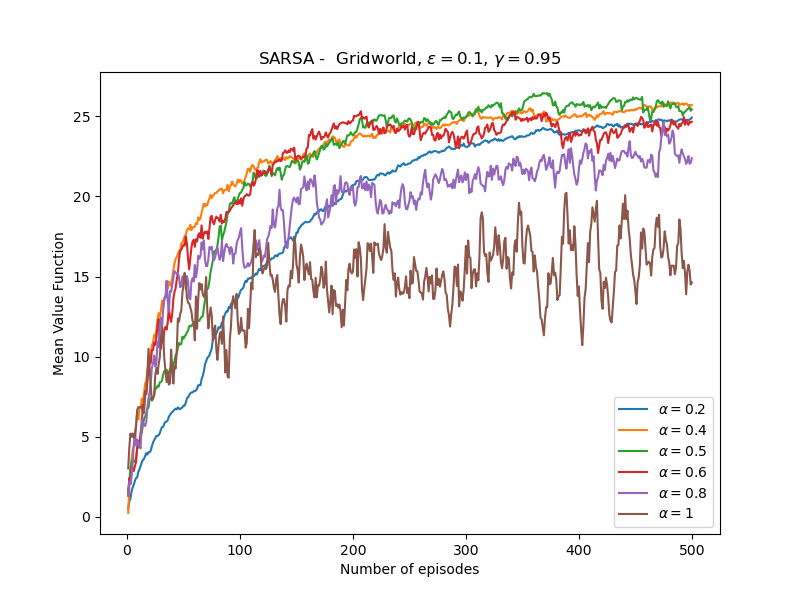
\includegraphics[width=3.5in]{g_sarsa_learning_curves_alpha}}
\caption{Learning Curve for Various Learning Rate ($\alpha$)}
\label{fig}
\end{figure}
\FloatBarrier

\begin{figure}[!htbp]
\centerline{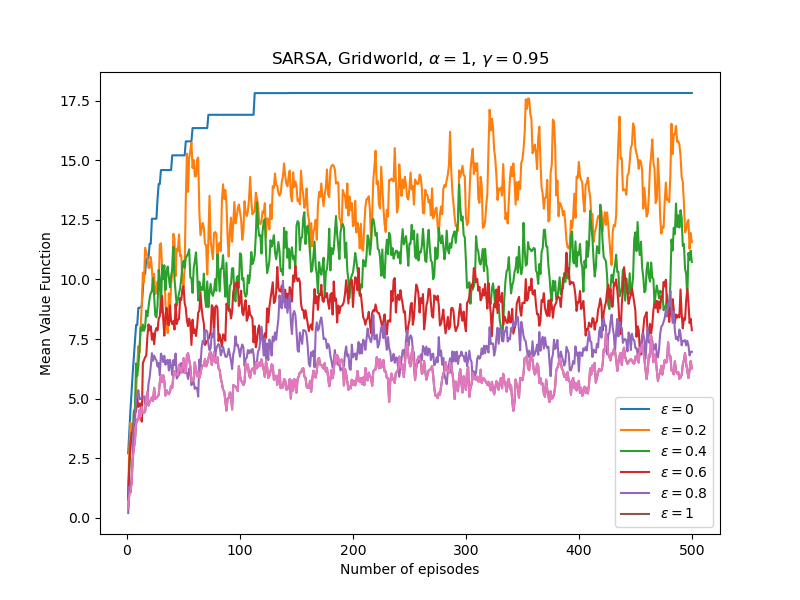
\includegraphics[width=3.5in]{g_sarsa_learning_curves_epsilon}}
\caption{Learning Curve for Various ($\epsilon$)}
\label{fig}
\end{figure}
\FloatBarrier

\begin{figure}[!htbp]
\centerline{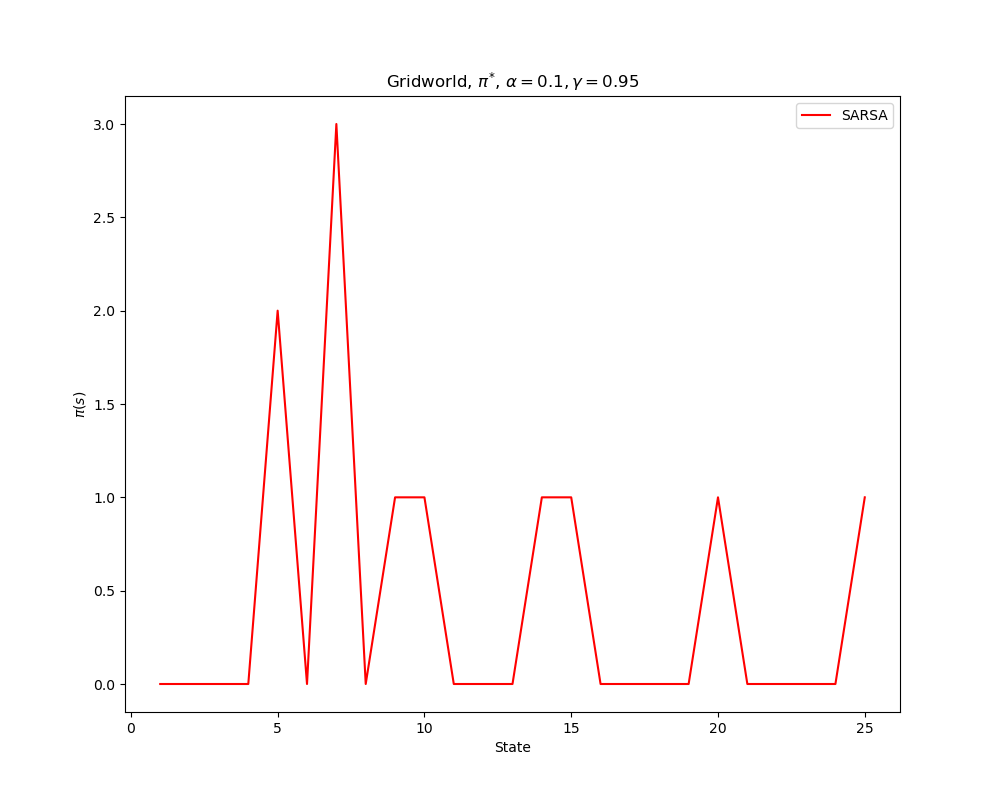
\includegraphics[width=3.5in]{g_sarsa_policy}}
\caption{Action-Value Function vs. Number of Episodes}
\label{fig}
\end{figure}
\FloatBarrier

\begin{figure}[!htbp]
\centerline{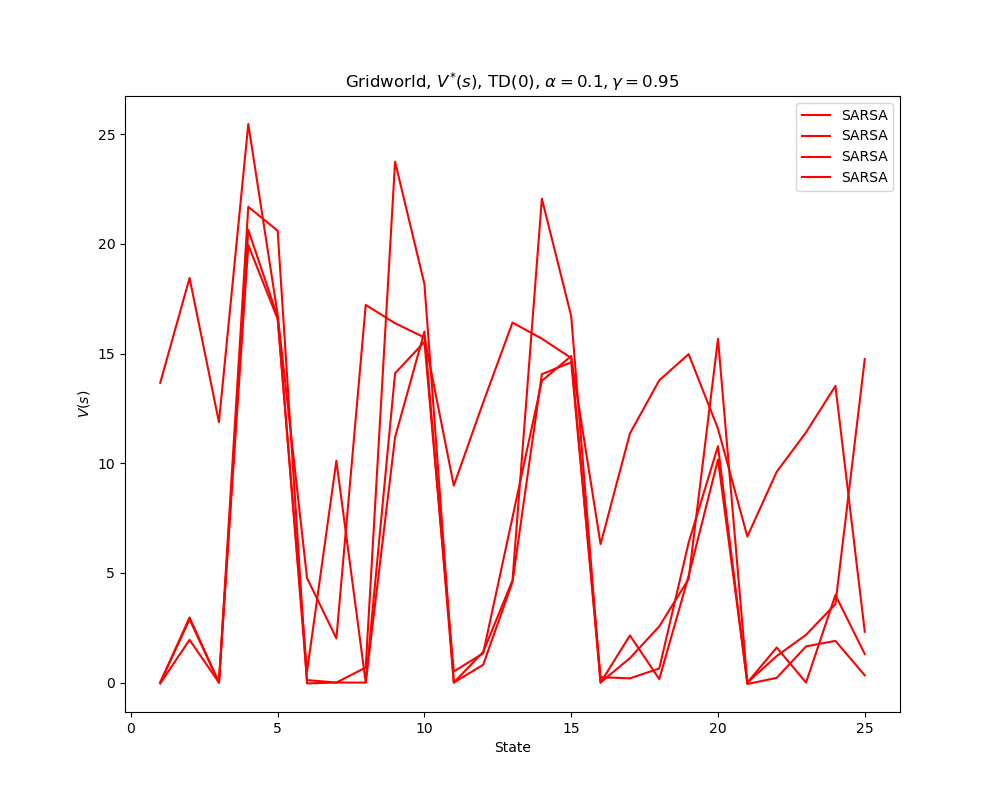
\includegraphics[width=3.5in]{g_sarsa_state_value}}
\caption{State-Value Function vs. Number of Episodes}
\label{fig}
\end{figure}
\FloatBarrier

\begin{figure}[!htbp]
\centerline{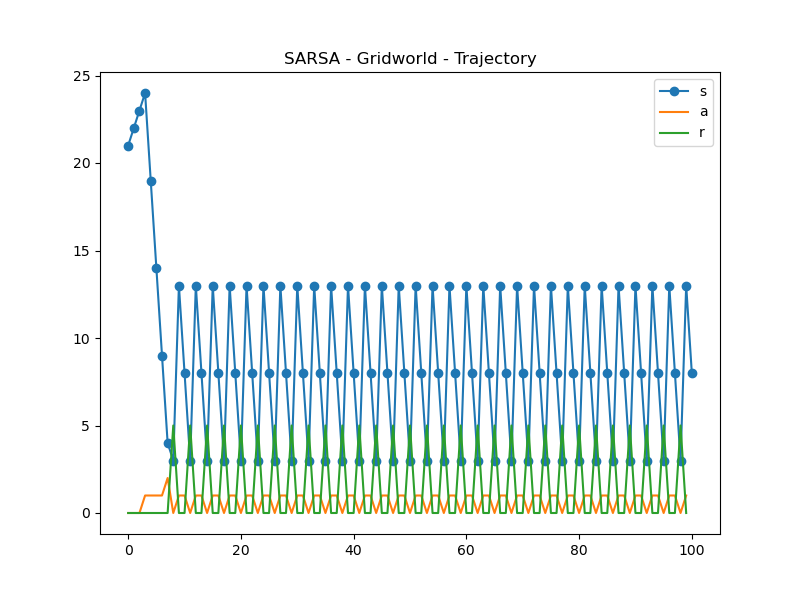
\includegraphics[width=3.5in]{g_sarsa_policy_vs_trajec}}
\caption{Policy vs. Trajectory}
\label{fig}
\end{figure}
\FloatBarrier

\subsection{Q-Learning}

Q-learning is a model-free reinforcement learning algorithm that learns an optimal policy without knowledge of the environment's dynamics. It estimates the optimal action-value function by iteratively updating Q-values based on experience gained through exploration. \cite{b1}

\begin{figure}[!htbp]
\centerline{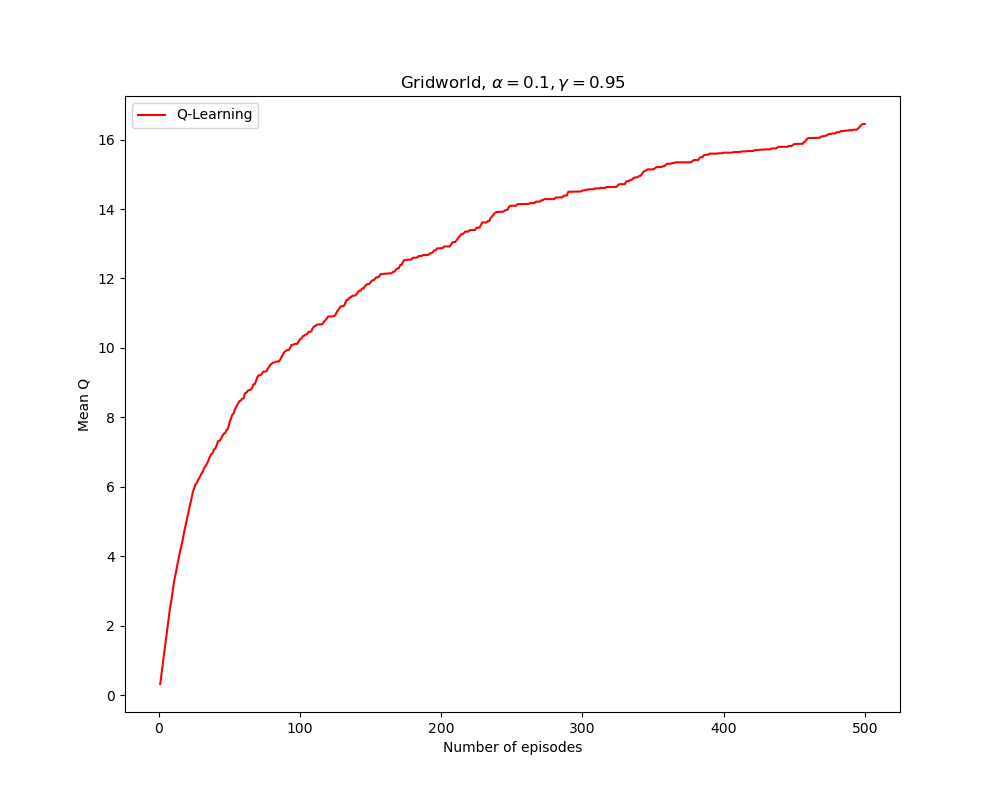
\includegraphics[width=3.5in]{g_ql_learning_curve}}
\caption{Learning Curve - Mean Value Function vs. Number of Episodes}
\label{fig}
\end{figure}
\FloatBarrier

\begin{figure}[!htbp]
\centerline{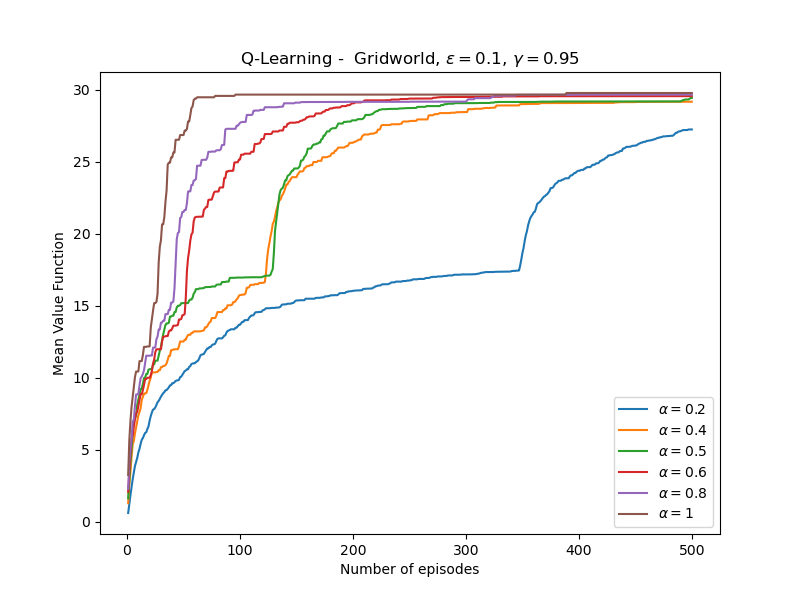
\includegraphics[width=3.5in]{g_ql_learning_curves_alpha}}
\caption{Learning Curve for Various Learning Rate ($\alpha$)}
\label{fig}
\end{figure}
\FloatBarrier

\begin{figure}[!htbp]
\centerline{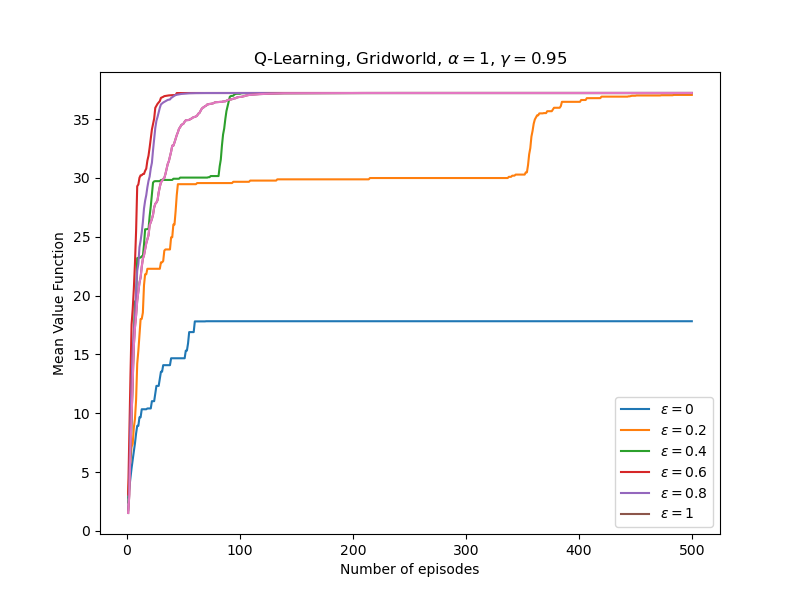
\includegraphics[width=3.5in]{g_ql_learning_curves_epsilon}}
\caption{Learning Curve for Various ($\epsilon$)}
\label{fig}
\end{figure}
\FloatBarrier

\begin{figure}[!htbp]
\centerline{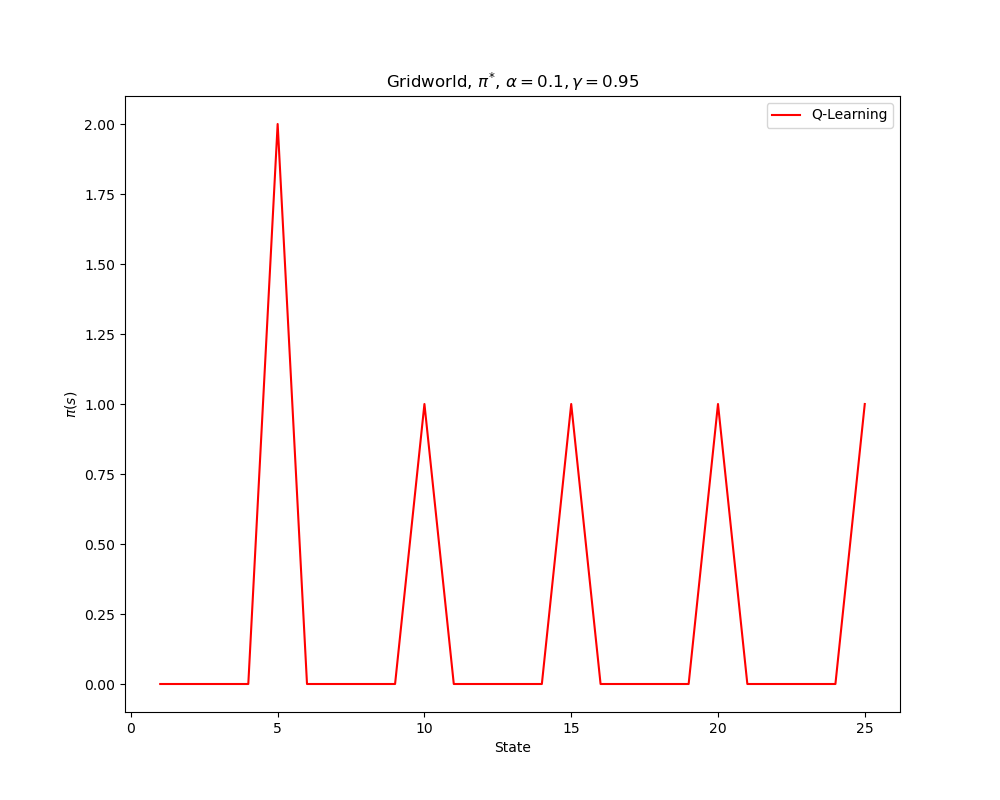
\includegraphics[width=3.5in]{g_ql_policy}}
\caption{Action-Value Function vs. Number of Episodes}
\label{fig}
\end{figure}
\FloatBarrier

\begin{figure}[!htbp]
\centerline{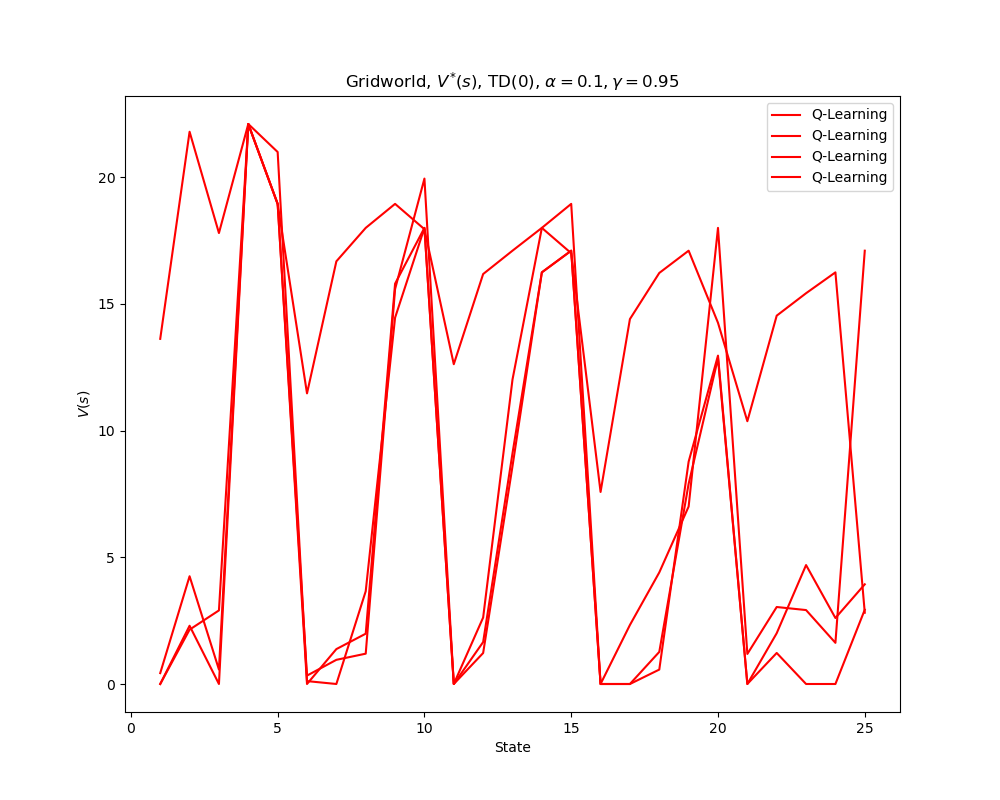
\includegraphics[width=3.5in]{g_ql_state_value}}
\caption{State-Value Function vs. Number of Episodes}
\label{fig}
\end{figure}
\FloatBarrier

\begin{figure}[!htbp]
\centerline{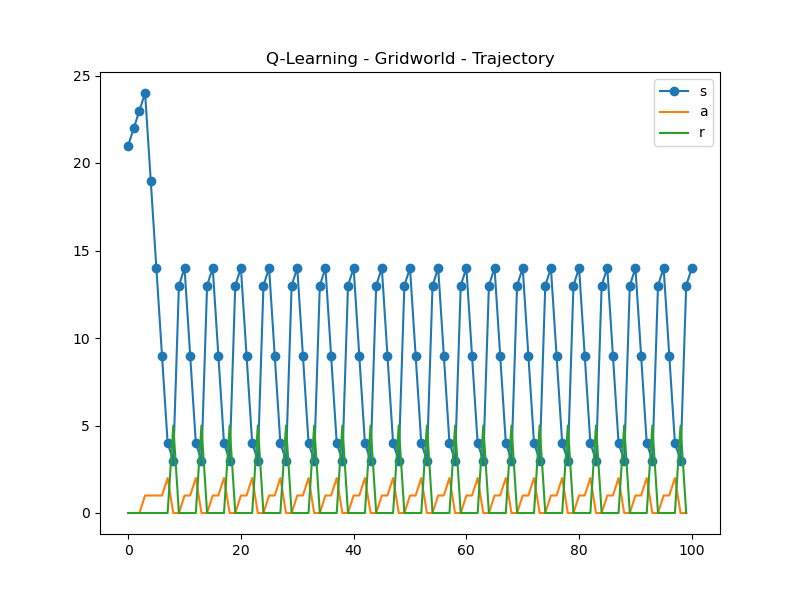
\includegraphics[width=3.5in]{g_ql_policy_vs_trajec}}
\caption{Policy vs. Trajectory}
\label{fig}
\end{figure}
\FloatBarrier

\section{Simple Pendulum}

\subsection{SARSA}

\begin{table}[h]
\caption{Hyperparameter values}
\renewcommand{\arraystretch}{1.5}
\centering
\begin{tabular}{|c|c|c|c|c|}
\hline
\textbf{Hyperparameter} &  \textbf{Values}  \\ \hline
\textbf{Gamma ($\gamma$)} & 0.95  \\ \hline
\textbf{Epsilon ($\epsilon$)} & 0 - 1  \\ \hline
\textbf{Alpha ($\alpha$)} & 0.2 - 1  \\ \hline
\textbf{Iterations} & 100 \\ \hline
\textbf{Episodes} & 500  \\ \hline
\textbf{Threshold ($\theta$)} & 1e-8 \\ \hline
\end{tabular} \\
\label{tab:hyperparameters}
\end{table}

\begin{figure}[!htbp]
\centerline{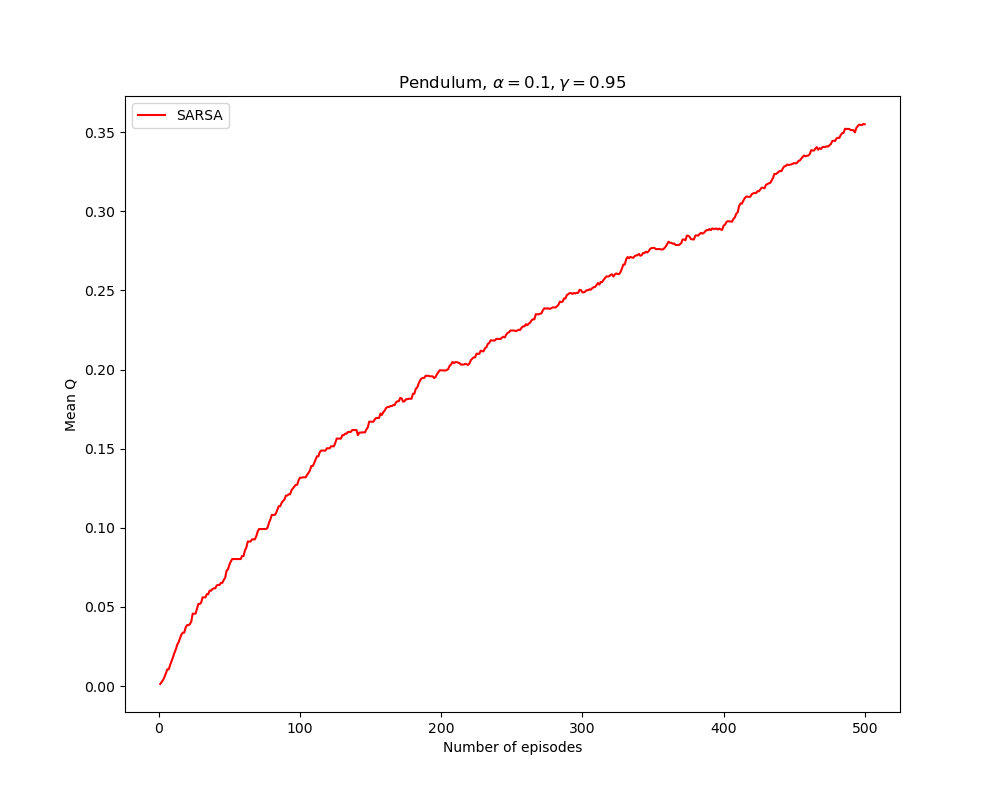
\includegraphics[width=3.5in]{p_sarsa_learning_curve}}
\caption{Learning Curve - Mean Value Function vs. Number of Episodes}
\label{fig}
\end{figure}
\FloatBarrier

\begin{figure}[!htbp]
\centerline{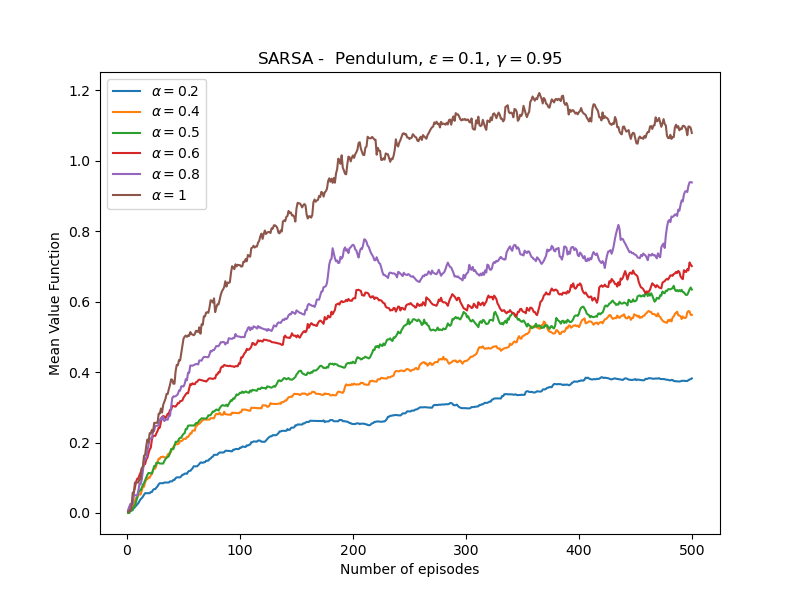
\includegraphics[width=3.5in]{p_sarsa_learning_curves_alpha}}
\caption{Learning Curve for Various Learning Rate ($\alpha$)}
\label{fig}
\end{figure}
\FloatBarrier

\begin{figure}[!htbp]
\centerline{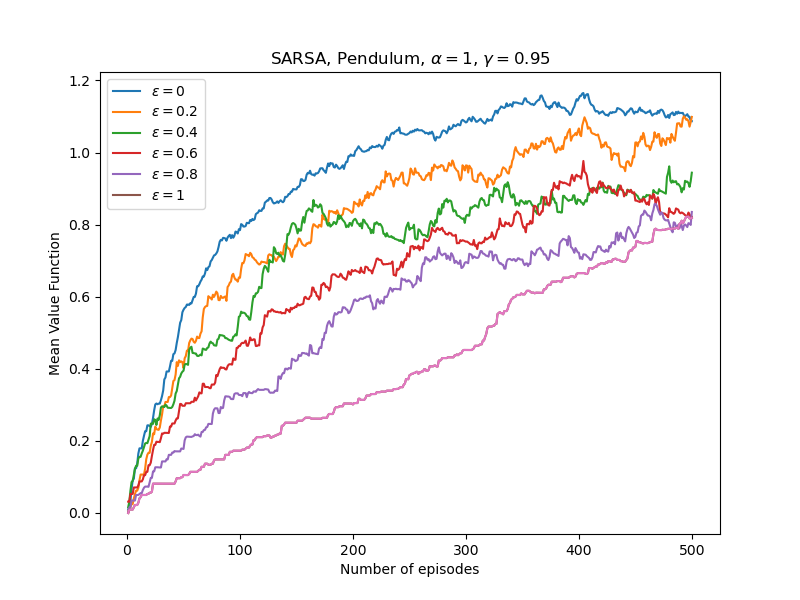
\includegraphics[width=3.5in]{p_sarsa_learning_curves_epsilon}}
\caption{Learning Curve for Various ($\epsilon$)}
\label{fig}
\end{figure}
\FloatBarrier

\begin{figure}[!htbp]
\centerline{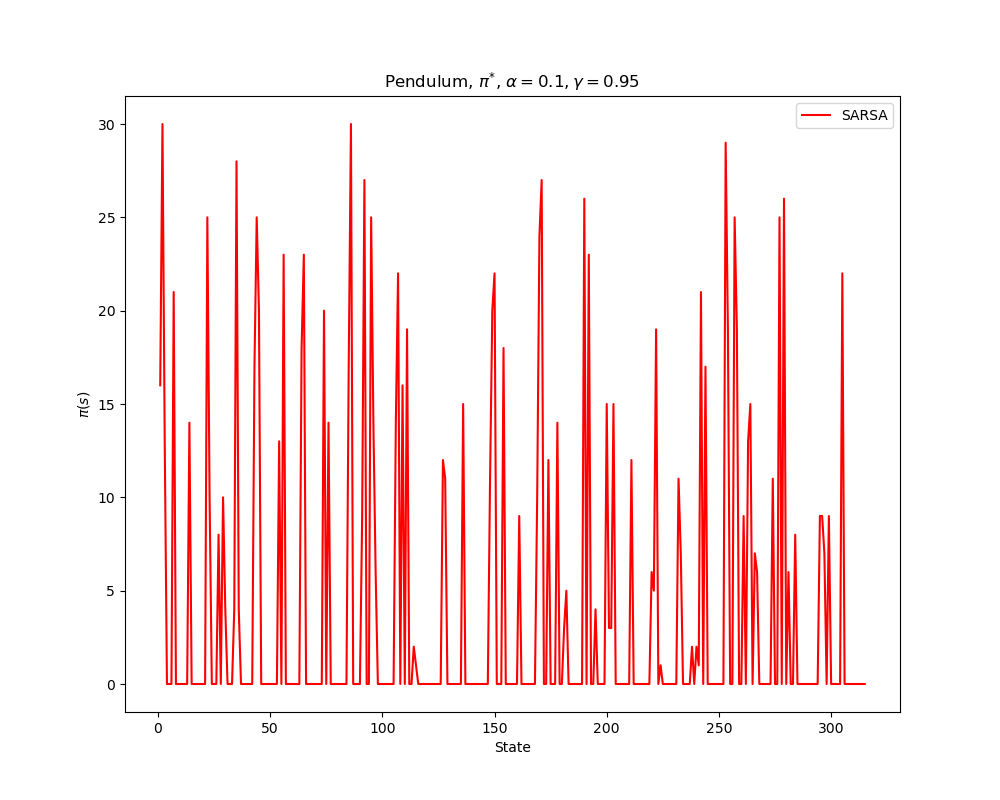
\includegraphics[width=3.5in]{p_sarsa_policy}}
\caption{Action-Value Function vs. Number of Episodes}
\label{fig}
\end{figure}
\FloatBarrier

\begin{figure}[!htbp]
\centerline{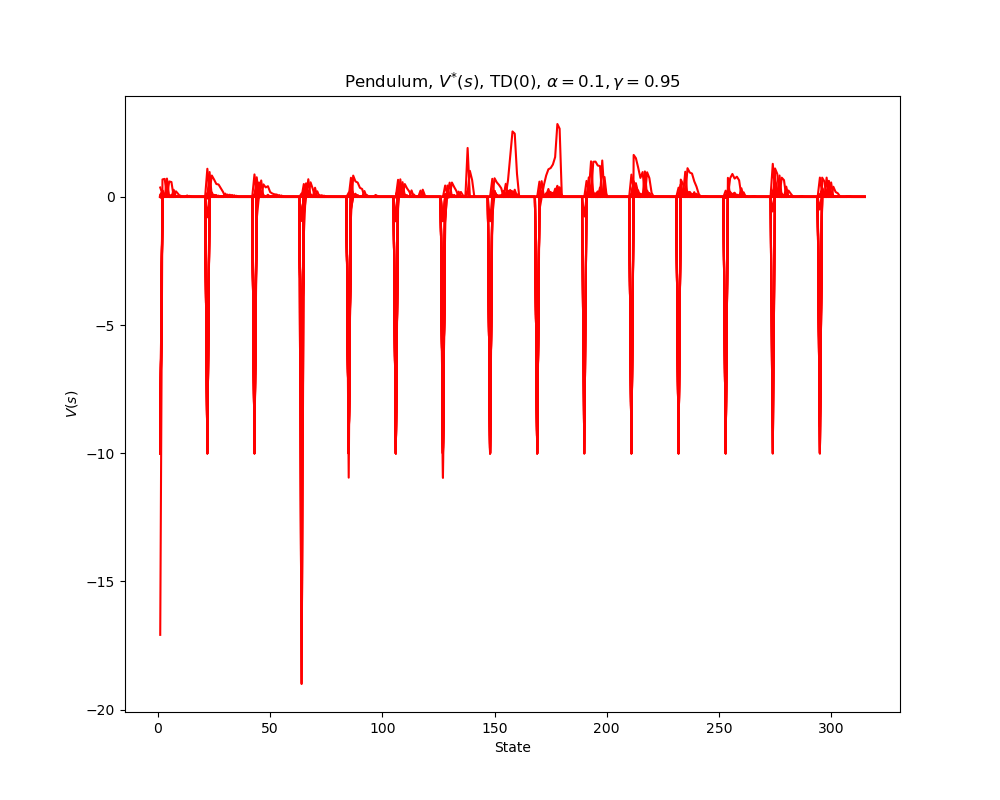
\includegraphics[width=3.5in]{p_sarsa_state_value}}
\caption{State-Value Function vs. Number of Episodes}
\label{fig}
\end{figure}
\FloatBarrier

\begin{figure}[!htbp]
\centerline{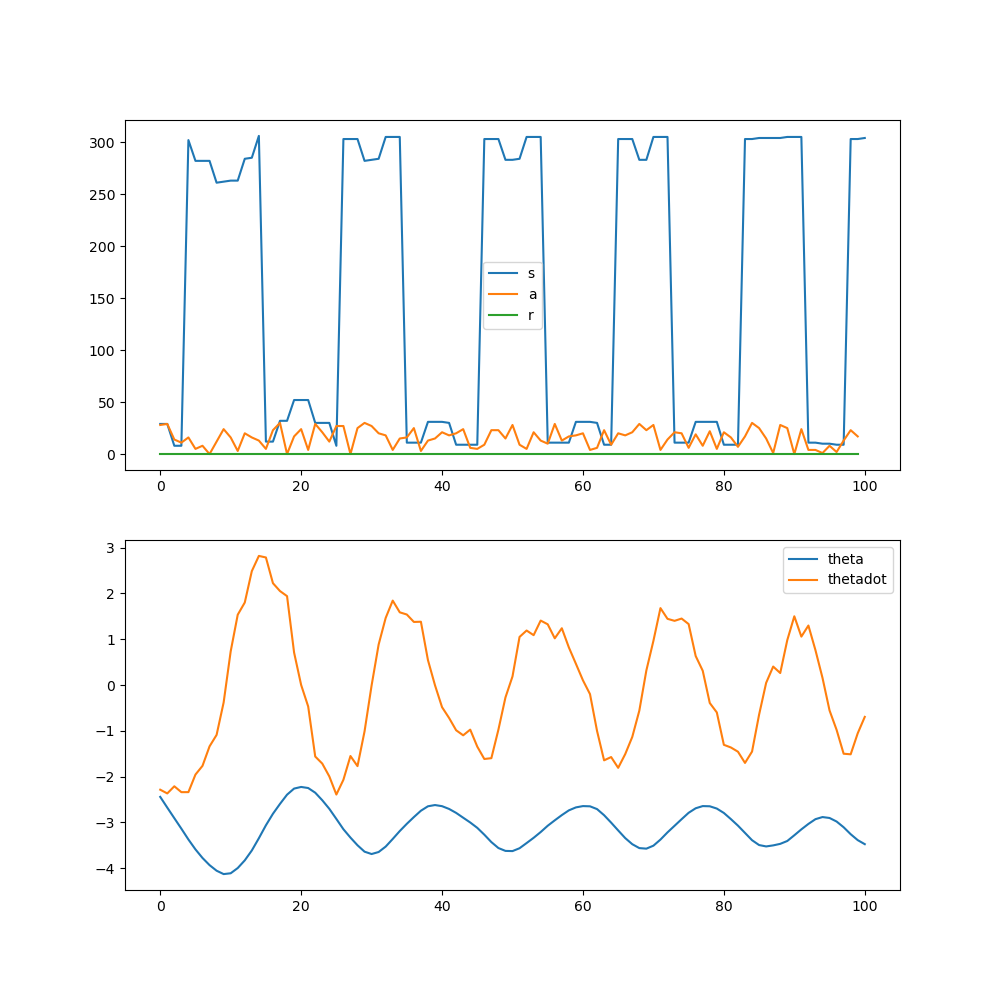
\includegraphics[width=3.5in]{p_sarsa_policy_vs_trajec}}
\caption{Policy vs. Trajectory}
\label{fig}
\end{figure}
\FloatBarrier

\subsection{Q-Learning}

\begin{figure}[!htbp]
\centerline{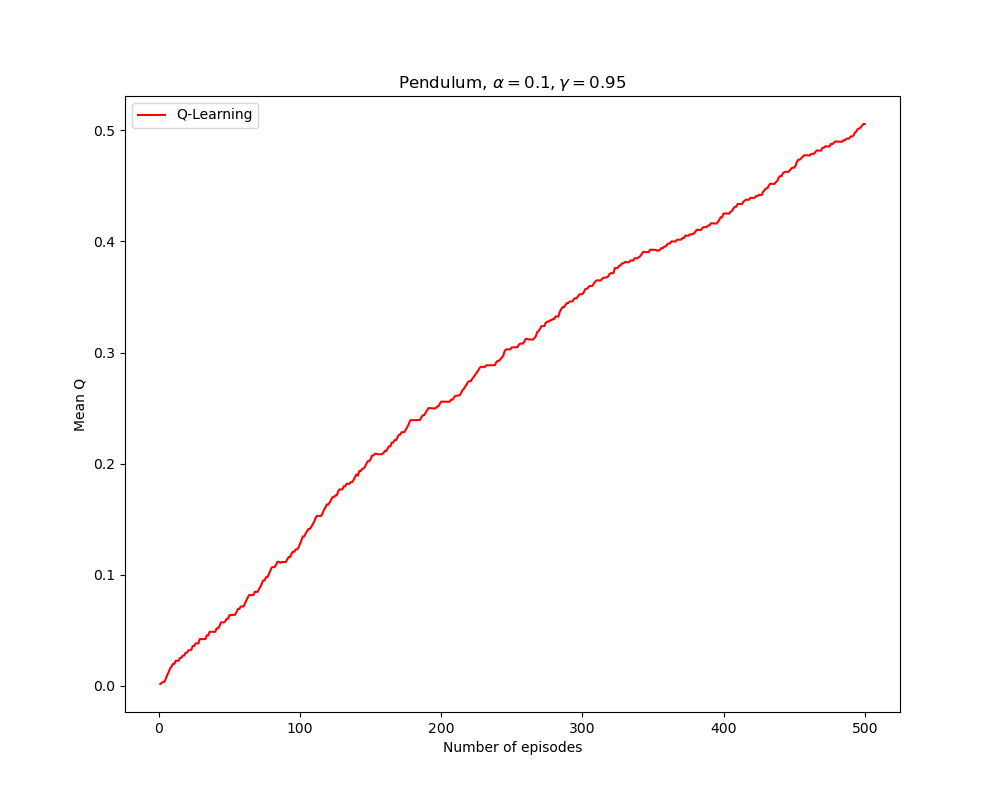
\includegraphics[width=3.5in]{p_ql_learning_curve}}
\caption{Learning Curve - Mean Value Function vs. Number of Episodes}
\label{fig}
\end{figure}
\FloatBarrier

\begin{figure}[!htbp]
\centerline{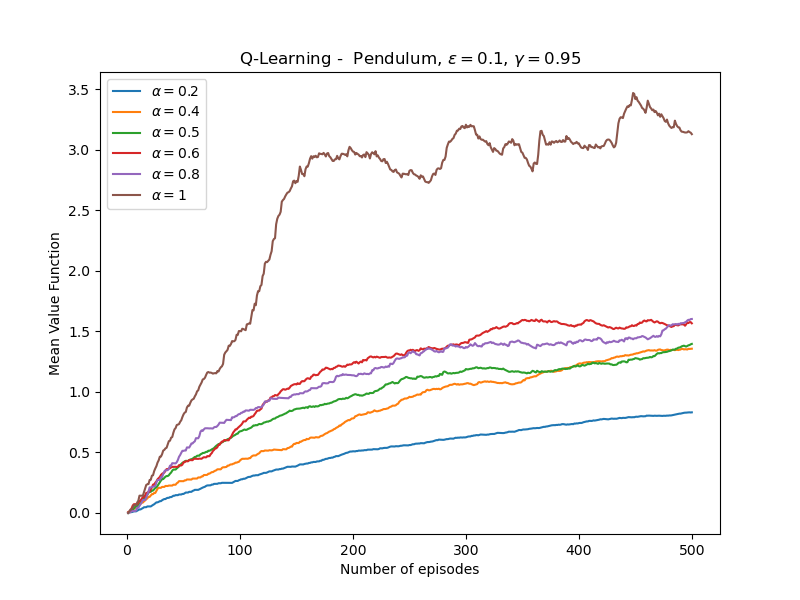
\includegraphics[width=3.5in]{p_ql_learning_curves_alpha}}
\caption{Learning Curve for Various Learning Rate ($\alpha$)}
\label{fig}
\end{figure}
\FloatBarrier

\begin{figure}[!htbp]
\centerline{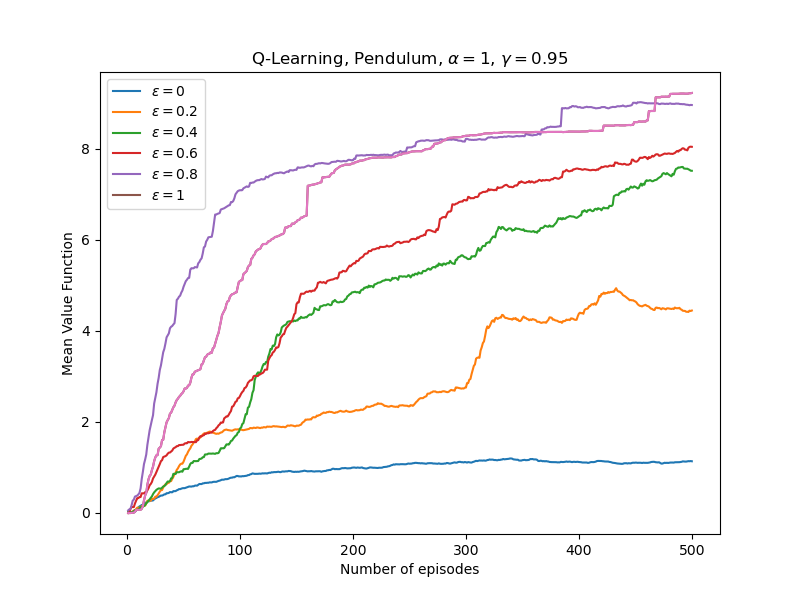
\includegraphics[width=3.5in]{p_ql_learning_curves_epsilon}}
\caption{Learning Curve for Various ($\epsilon$)}
\label{fig}
\end{figure}
\FloatBarrier

\begin{figure}[!htbp]
\centerline{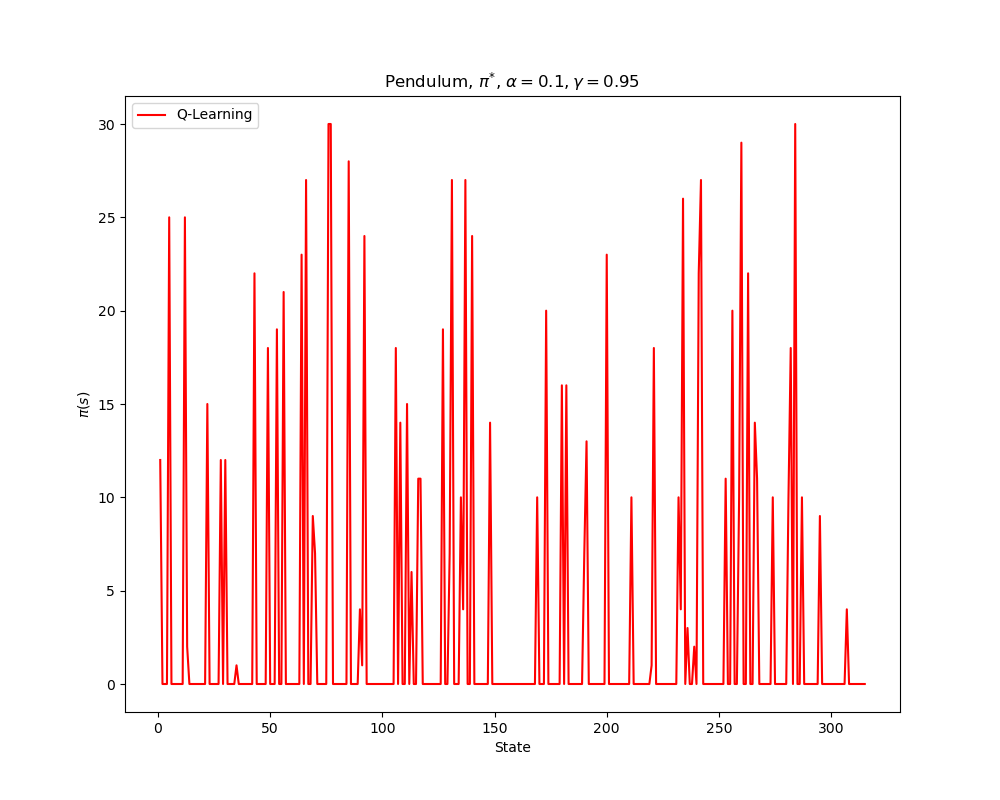
\includegraphics[width=3.5in]{p_ql_policy}}
\caption{Action-Value Function vs. Number of Episodes}
\label{fig}
\end{figure}
\FloatBarrier

\begin{figure}[!htbp]
\centerline{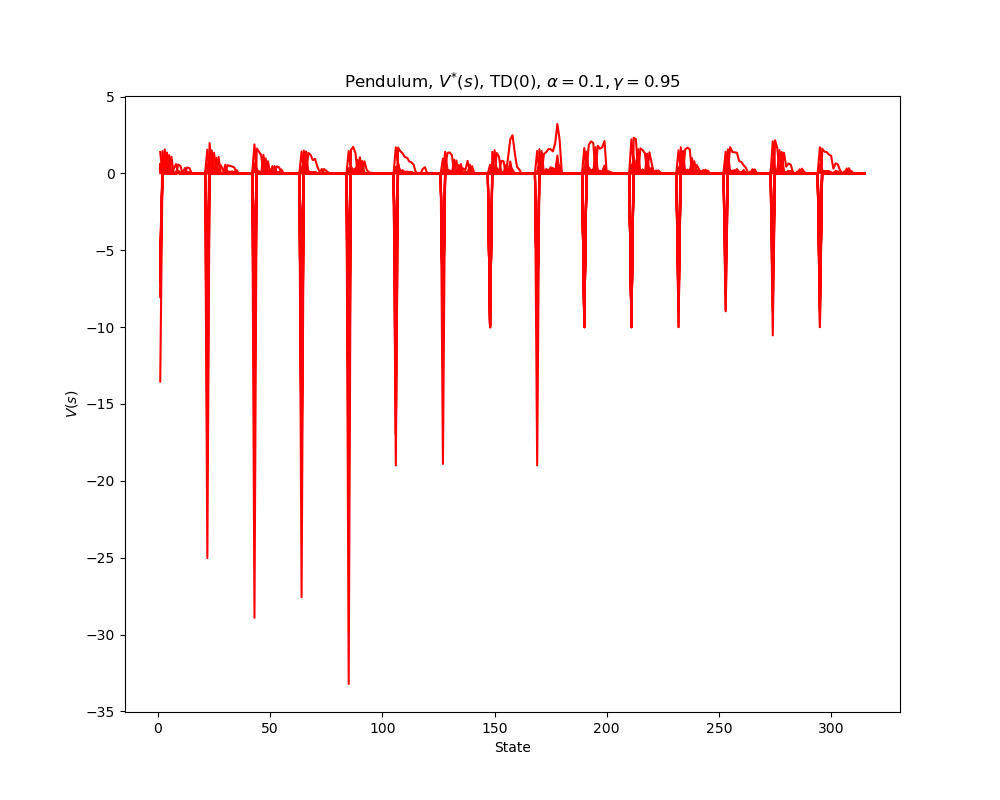
\includegraphics[width=3.5in]{p_ql_state_value}}
\caption{State-Value Function vs. Number of Episodes}
\label{fig}
\end{figure}
\FloatBarrier

\begin{figure}[!htbp]
\centerline{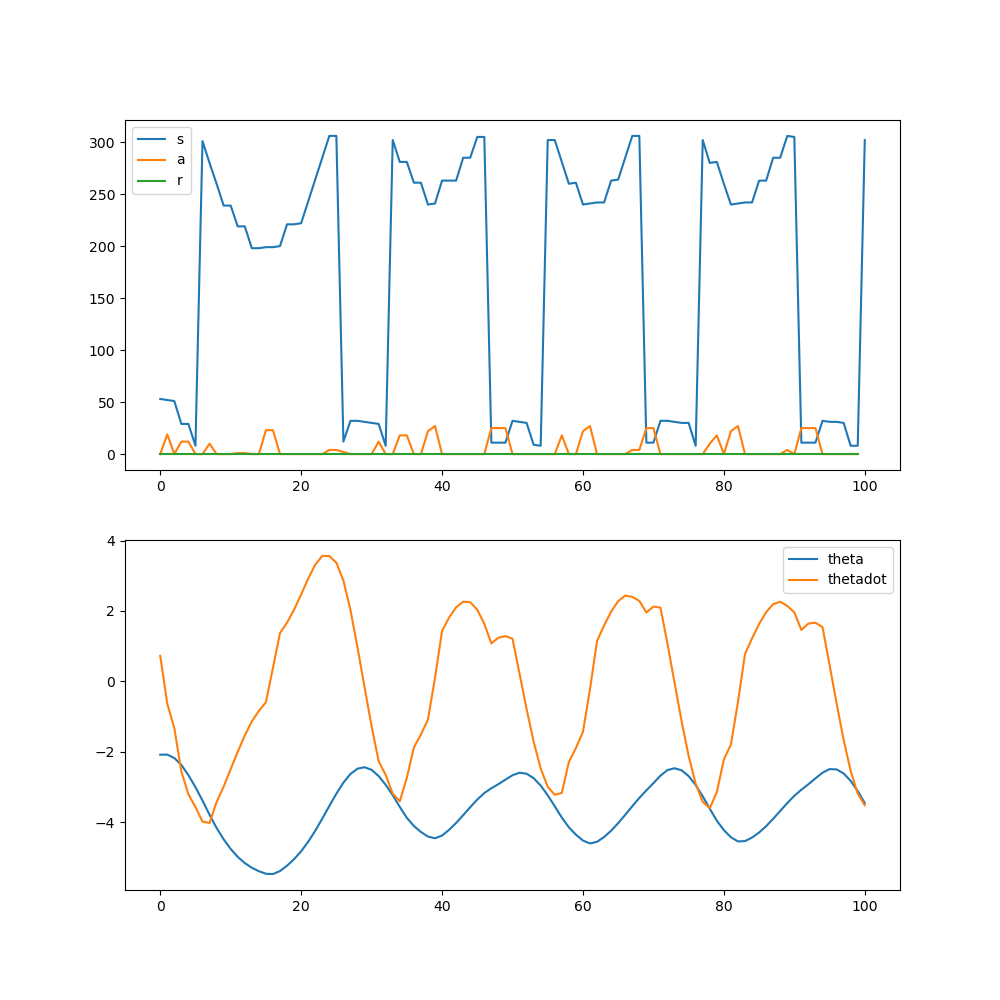
\includegraphics[width=3.5in]{p_ql_policy_vs_trajec}}
\caption{Policy vs. Trajectory}
\label{fig}
\end{figure}
\FloatBarrier

\begin{thebibliography}{00}
\bibitem{b1}  Sutton, R. S., and Barto, A. G. Reinforcement learning: An introduction (2nd ed.). The MIT Press. (2018)
\end{thebibliography}
\vspace{12pt}

\end{document}
